\documentclass[iop]{emulateapj}  % this makes everything look like ApJ
%\documentclass[12pt,preprint]{aastex}  % for e-submission to ApJ
%\documentclass[12pt,preprint2]{aastex}  % for e-submission to ApJ - two column
%\documentclass[manuscript]{emulateapj}  % this makes everything look like ApJ

\usepackage{graphicx, natbib, color, bm, amsmath, epsfig}

\citestyle{aa}  % correct formatting for ApJ style files

\begin{document}
\title{Parameter Space of CMB Foregrounds}
\author{Kye Stalpes \altaffilmark{1}, David Collins
\altaffilmark{1}, et al.}

\altaffiltext{1}{Department of Physics, Florida State University}

\begin{abstract}
Through numerical magnetohydrodynamical (MHD) simulations we examine the E/B
power spectra of the polarized multiphase interstellar medium (ISM) over a wide
swath of dust parameter space. We describe the relative importance of gas
pressure and magnetic field pressure on the shape of the E and B power spectra
recently observed by Planck in their search for the B-modes of primordial
gravitational waves in the polarized Cosmic Microwave Background (CMB). We describe our findings and how they impact our
understanding of the polarized dust foregrounds.
\end{abstract}

\keywords{methods: numerical --- AMR, MHD, CMB, Power Spectra, ISM}

\maketitle


%\tableofcontents
\section{Introduction}
The theory of inflation is a widely accepted theory of the origins of the early
universe in which space underwent a period of extremely rapid expansion
shortly after the big bang. This theory has been extremely successful in
explaining a wide range of cosmological problems yet direct confirmation thus
far has been elusive. Primordial gravitational waves created during the
inflationary epoch \citep{Starobinskii79, Kamionkowski15} and stretched to observable scales would imprint curl-like
B-modes on the polarized CMB \citep{Guth81, Linde82} and provide just such a direct confirmation.

Direct observation of these polarized signals are complicated by the presence of
the polarized dust foreground of the ISM and many recent efforts
\citep{Kritsuk17, Bracco19} have been
devoted to better understanding the properties of this foreground in order to
achieve the sensitivities needed to measure the primordial B-mode signal
characterized by the tensor-to-scalar ratio $r$ \citep{Baumann09, Planck15}. One
of the more promising results found by Planck's 353GHz waveband survey \citep{Planck15, Planck18XI} is that
the polarized dust foreground shows several consistent properties across the
high lattitude sky. In this paper we focus on exploring the observations that the ratio of
E-mode to B-mode power $r$ in the foreground dust spectra is ~2
\citep{Caldwell16, Planck18XI} and that both E and
B power spectra have a measured slope of ~-2.5 (specifically $\alpha_{EE}=-2.42$ and
$\alpha_{BB}=-2.54$) \citep{Planck15, Planck18XI}. We also
discuss the finding by \citep{Planck18XI} that the predicted T/E and T/B power
ratio of 0 is observed to be non-zero.

A linear polarization signal can be decomposed into two rotationally invariant
quantities, E (gradient/scalar) and B (curl/tensor) modes \citep{Kamionkowski97,
Zaldarriaga97}. Since random orientated or random amplitude fixed orientation
polarization signals would appear with equal E and B powers, the Planck finding
of an EE/BB power ratio ~2 implies some non-random coherence between the two signals
that must arise from underlying physics in the dust foreground.

The slopes of the power spectra reflect the amount of power at a given size
scale in the turbulent medium as energy cascades from the injection scale to the
dissipation scale (this gap being called the inertial range) where energy is
dissipated into the surrounding system, typically in the form of heat due to
viscocity. Several relatively recent works that explore these effects in more
detail are \citep{Clark14,Ghosh17,Cho02}. The slope of such a cascade in
the inertial range is dictated by several factors such as the sonic Mach number
$M_{s}$ which is the ratio of flow velocity to the speed of sound in the gas and
the Alfven Mach number $M_{a}$ which is the ratio of the flow velocity to the
Alfven velocity. The Alfven velocity is the speed of a particular type of
oscillation of plasma ions in a magnetic field and is dictated by the magnetic
field strength and the gas density. Finding the correct combination of Mach
number and Alfven Mach number to allow for spectral slopes in E and B of
$\alpha=~-2.5$ \citep{Planck18XI} reveals important information on the properties of the polarized foreground.


\section{Simulations and Analysis}

\subsection{MHD Equations}
These simulations are done using the open source code Enzo (\citet{Bryan14}) to
solve the Eulerian equations of ideal magnetohydrodynamics (MHD) using the
method of adaptive mesh refinement (AMR) to achieve the dynamic resolution scales
needed for this type of problem. These MHD equations (as can be found in the
Enzo documentation cited above) with no gravity are shown below in cgs
units with magnetic permeability set to 1.   

\begin{equation} \label{eq:MHD1}
    \frac{\partial \rho}{\partial t}
+ \nabla \cdot
(\rho \mathbf{v})
= 0
\end{equation}
\begin{equation} \label{eq:MHD2}
    \frac{\partial \rho \mathbf{v} }{\partial t}
+ \nabla \cdot
\left(
        \rho \mathbf{v} \mathbf{v}
        + \mathbf{I} P
        - \frac { \mathbf{B} \mathbf{B} }{ 8 \pi }
\right)
=
0
\end{equation}
\begin{equation} \label{eq:MHD3}
\frac{\partial E}{\partial t}
+ \nabla \cdot
\left[
        (E + P) \mathbf{v}
        -
        \frac
        { \mathbf{B} ( \mathbf{B} \cdot \mathbf{v} ) }
        { 4 \pi }
\right]
= 0
\end{equation}
\begin{equation} \label{eq:MHD4}
\frac {\partial \mathbf{B} }{\partial t}
- \nabla \times ( \mathbf{v} \times \mathbf{B})
=0
\end{equation}


where $\mathbf{v}\mathbf{v}$ and $\mathbf{B}\mathbf{B}$ are
the velocity and the magnetic field outer products, $\phi$ is
the density,$\Lambda$ and $\Gamma$ represent
radiative cooling and heating and $\mathbf{F}_{cond}$ is the flux due to thermal
heat conduction.
The total energy density  is
equal to the total of the kinetic,
the thermal and the magnetic energy,

\begin{equation} \label{eq:E-total}
E = e + \frac{ \rho v^2 }{ 2 } + \frac{B^2}{8\pi}
\end{equation}

and

\begin{equation} \label{eq:P-total}
P = p + \frac{B^2}{8\pi}
\end{equation}

is the total thermal plus the magnetic pressure.

The system is closed by an equation of state.

\begin{equation} \label{eq:EOS}
e = \frac{p}{\gamma - 1}
\end{equation}

where the equation of state is shown for an ideal gas with a ratio of specific
heats $\gamma$.
\subsection{Adaptive Mesh Refinement}
The difficult problem mentioned before of large dynamic spatial and temporal
scales inherent to this study is handled through the implementation of adaptive
mesh refinement (AMR). This method actively increases and decreases the 
local mesh resolution and time step based on desired local parameters such as
Jean's length, metalicity or density. This enables us to conserve computational
power on regions that are largely static and direct it toward the dynamic, dense
regions that are evolving rapidly on the galactic time scales. This method often
enables us to achieve effective resolutions several orders of magnitude larger
than would be possible using a fixed grid with a similar computational time
while losing very little accuracy in the coarse regions. 

When running our simulation we select several criteria (such as those outlined
above) that will 'flag' a region as requiring increased grid resolution or
shorter time steps in order to achieve the desired accuracy. This region is then
subdivided into several smaller regions that the equations can be solved on. If
the smaller regions no longer satisfy the 'flagged' criterion they are solved
and the entire simulation moves forward. If any zone within this new region is
still being flagged then it too is subdivided and rechecked until either an
appropriate resolution is achieved or it reaches the maximum resolution defined
manually in the code at which point it is solved as is. 

\subsection{Simulation Parameters}

These simulations use a root grid of $512^{3}$ with two levels of refinement to
yield an effective resolution of $2048^{3}$. The sonic Mach number $M_{s}$ and
Alfven Mach number $M_{a}$ are chosen here to be $$M_{s} = 0.5, 1, 2, 3$$ and
$$M_{a} = 0.5, 1, 2$$ across the suite of 12 simulations designed to probe the
polarized dust parameter space.

Here I need to list all the important parameter values such as $\rho_0$ the
ratio of solenoidal to compressible turbulence, gamma, blah blah.

The box is driven by ??purely solenoidal turbulence?? throughout the simulation and
allowed to run for 10 crossing times $t_{cross}$. The data presented in this
paper is taken from times between 5 to 10 $t_{cross}$ to ensure that a
statistically relaxed state has been reached before analysis is begun.

\subsection{Synthetic Observations}

When we speak of synthetic measurements we are referring to the ability to
use simulations (or numerical methods in general) to reproduce measurements or
data in the same way that it is collected and analyzed by physical observers.
For instance this may refer to generating 2-D projected column density maps
based on a luminosity distance relationship as opposed to looking at the 3-D
density field value at a given point. It should come as no surprise that the
majority of synthetic measurements will involve the observation of sources in
emission. There are however some cases of interest to us such as extinction
mapping in the ISM where absorption maps will also play an important role.

In this work we analyze synthetic polarization dust maps in order to gain a
better insight into the relationship between the underlying physical
information, and it presents itself to observers. This is important since
ultimately we are comparing our results with values seen on the real sky.


\section{Methodology}




\section{E and B Power Spectra Slopes}

To probe the possible parameter space that gives rise to the observed EE and BB spectral
slopes reported by \citep{Planck18XI} we run our simulations through a range of
sonic $M_s$ and Alfven $M_a$ Mach numbers over the course of 12 separate
simulations at a resolution of $512^3$. Functionally this means that we have
simulations of varying initial magnetic field strengths $B_{rms}$ and rms gas
velocities $v_{rms}$ which may (and do) evolve throughout the course of the
simulation. We then plot the EE and BB power spectra and fit the slope within
the most likely inertial range (within the injection and dissapation scale).

\begin{figure}[h]
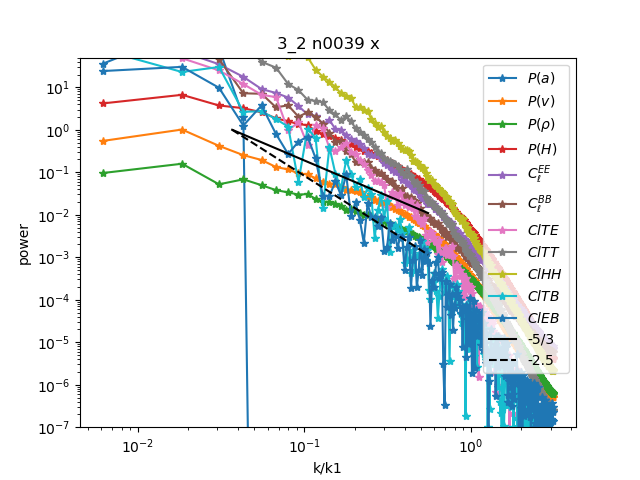
\includegraphics[width=\linewidth]{3_2_spectra_0039_x.png}
\caption{Example power spectra shown for various quantities at $M_s=3$ and
$M_a=2$ with line of sight along the magnetic field in a well evolved state
toward the end of the simulation run. Overplotted are the expected -2.5 slopes
for EE and BB observed by Planck et al. as well as the -5/3 slope which would be
observed for homogeneous self-similar Kolmogorov turbulence.}
\label{fig:example_spectra}
\end{figure}

In figure ~\ref{fig:example_spectra} we see a typical result for the observed
power spectra from various quantities in our simulation in a given run. In this
super-Alfvenic, super-sonic run we can observe the flatter left-most part of the
spectra corresponding to the injection scale, the relatively constant sloping
inertial range from which our measured slopes are drawn and the steeply sloped
dissapation scale toward the bottom-right of our spectra. 

\begin{figure}[h]
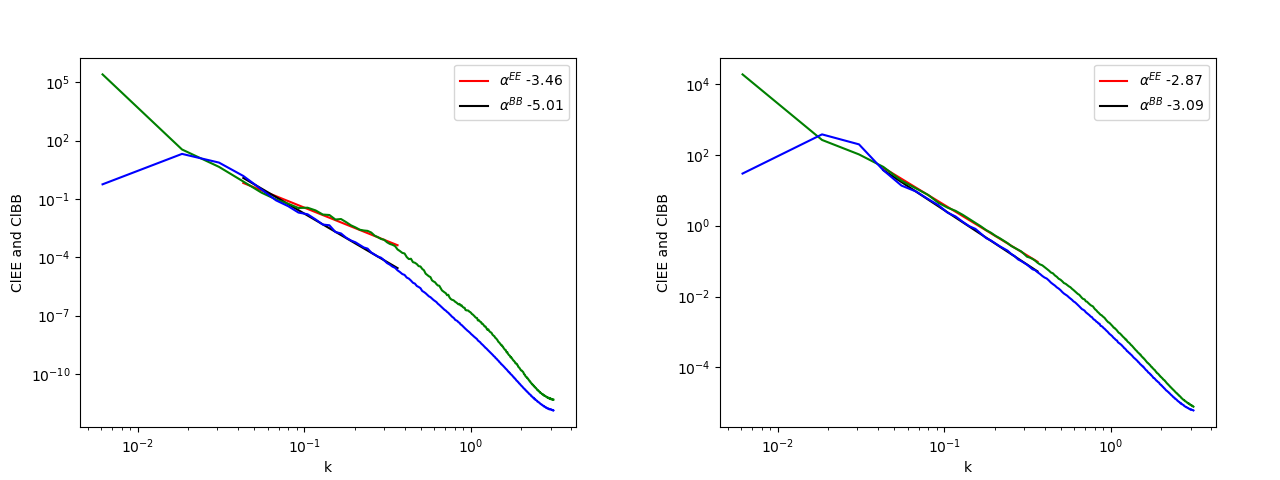
\includegraphics[width=\linewidth]{half_half_to_3_2_spectra_y.png}
\caption{Above we see how the EE (green line/red slope) and BB (blue line/black
slope) spectra change between a sub-sonic
($M_s=0.5$) sub-Alfvenic ($M_a=0.5$) (left-most image) and a super-sonic
($M_s=3$) super-Alfvenic ($M_a=2$) (right-most image) run.}
\label{fig:half_half_3_2_spectra}
\end{figure}

Looking specifically at the EE and BB power spectra we see in figure
~\ref{fig:half_half_3_2_spectra} generically that the spectra and their
respective slopes are largely influenced by the local values of $M_s$ and
$M_a$. Indeed the right-most image exhibits slopes much closer to the -2.5
values observed by the Planck collaboration. 

\begin{figure}[h]
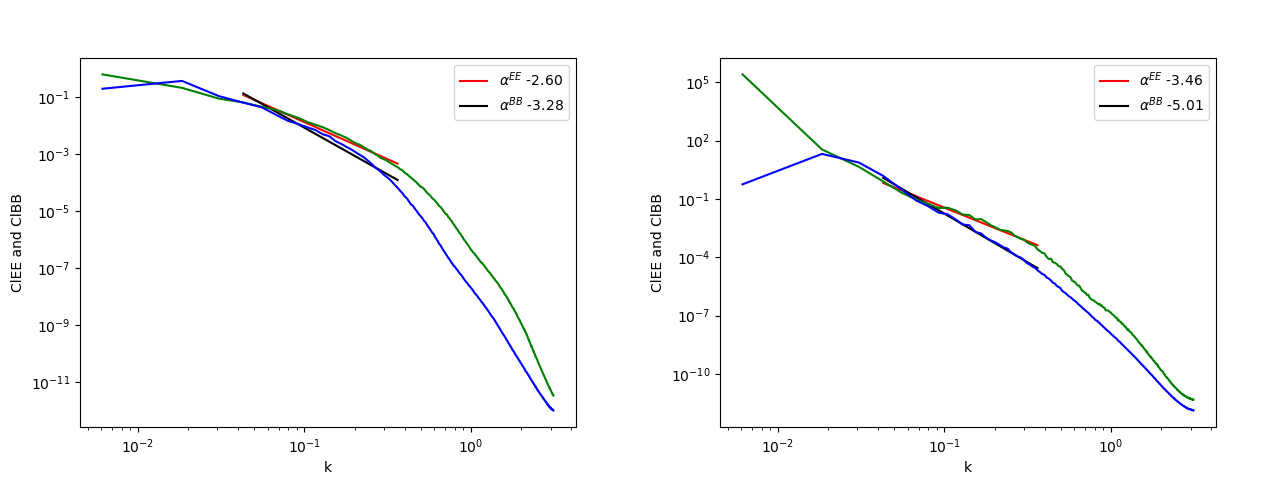
\includegraphics[width=\linewidth]{half_half_spectra_x_y.png}
\caption{The above figure shows how the EE (green line/red slope) and BB (blue line/black
slope) spectra can change for a given run between lines of sight. This sub-sonic
($M_s=0.5$) sub-Alfvenic ($M_a=0.5$) run image shows spectra observed with line of sight along the
background magnetic field (left-most image) and transverse to the field
(right-most image).}
\label{fig:half_half_los_spectra}
\end{figure}

Perhaps unsurprisingly we also find that the shape of the power spectra can be
strongly influenced by line of sight orientation relative to the direction of
the background magnetic field. This effect is most pronounced in the strong
field (low $M_a$) weak gas pressure (low $M_s$) runs where the magnetic pressure
dominates the flow. In figure ~\ref{fig:half_half_los_spectra} we can see two
very distinct EE and BB spectra taken from the same $M_s=0.5$ $M_a=0.5$
simulation run when looked at from lines of sight parallel (left image) and
transverse (right image) to the background magnetic field. When discussing the
results of our paramater space sampling on the observed slopes between runs we
must be careful to acknowledge the effect this has on the overall conclusions
drawn.

\begin{figure}[h]
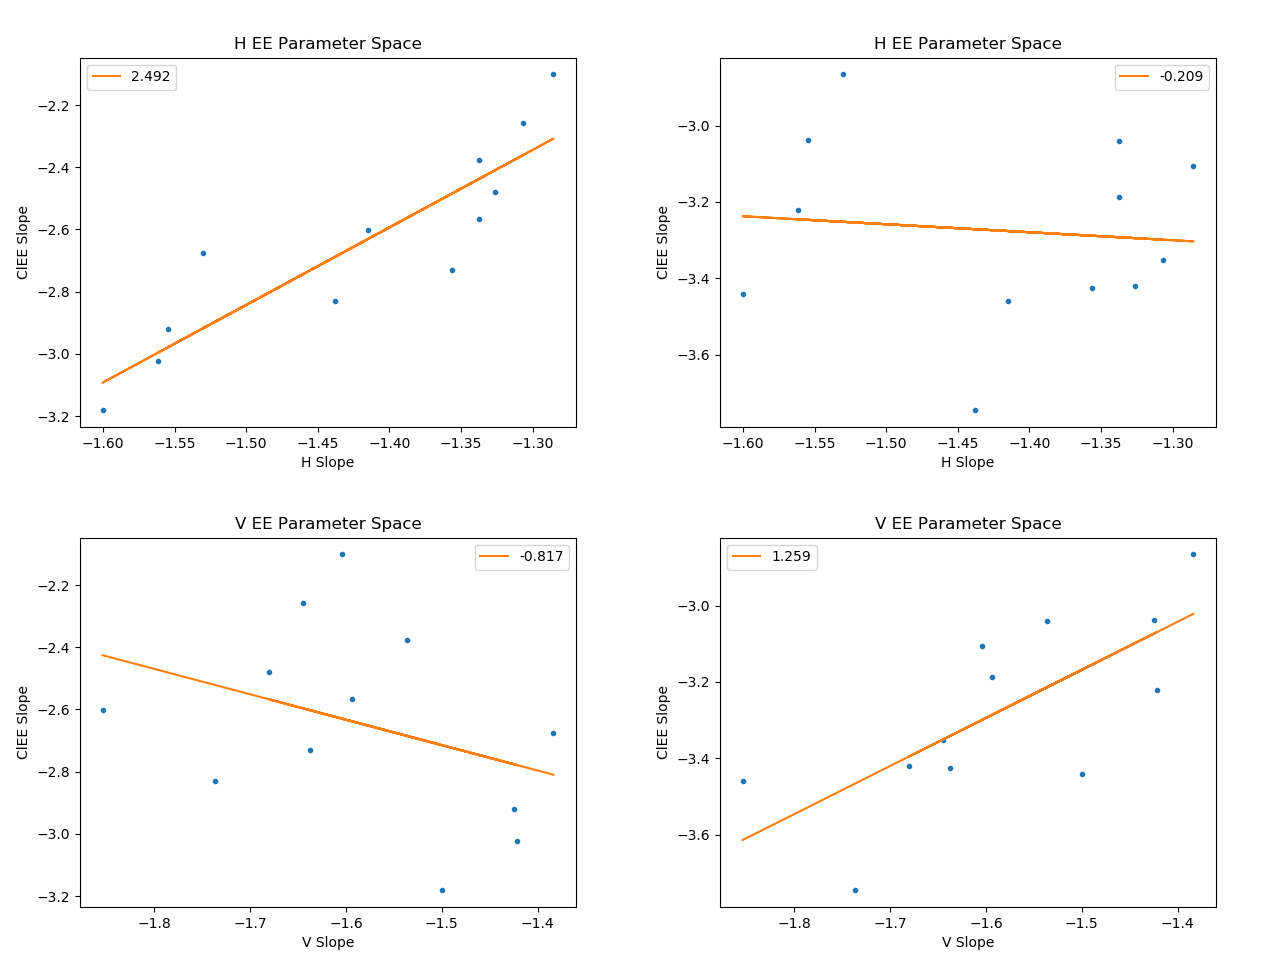
\includegraphics[width=\linewidth]{ee_V_H_x_y_paramspace.png}
\caption{Top Left: Slope of EE power spectra vs. slope of H-field spectra with
line of sight parallel to H-field. Top Right: Slope of EE power spectra vs. slope of H-field spectra with los transverse to H-field. Bottom Left: Slope of EE power spectra vs. slope of
velocity spectra with los parallel to H-field. Bottom Right: Slope of EE power spectra vs.
slope of velocity spectra with los transverse to H-field}
\label{fig:ee_V_H}
\end{figure}

\begin{figure}[h]
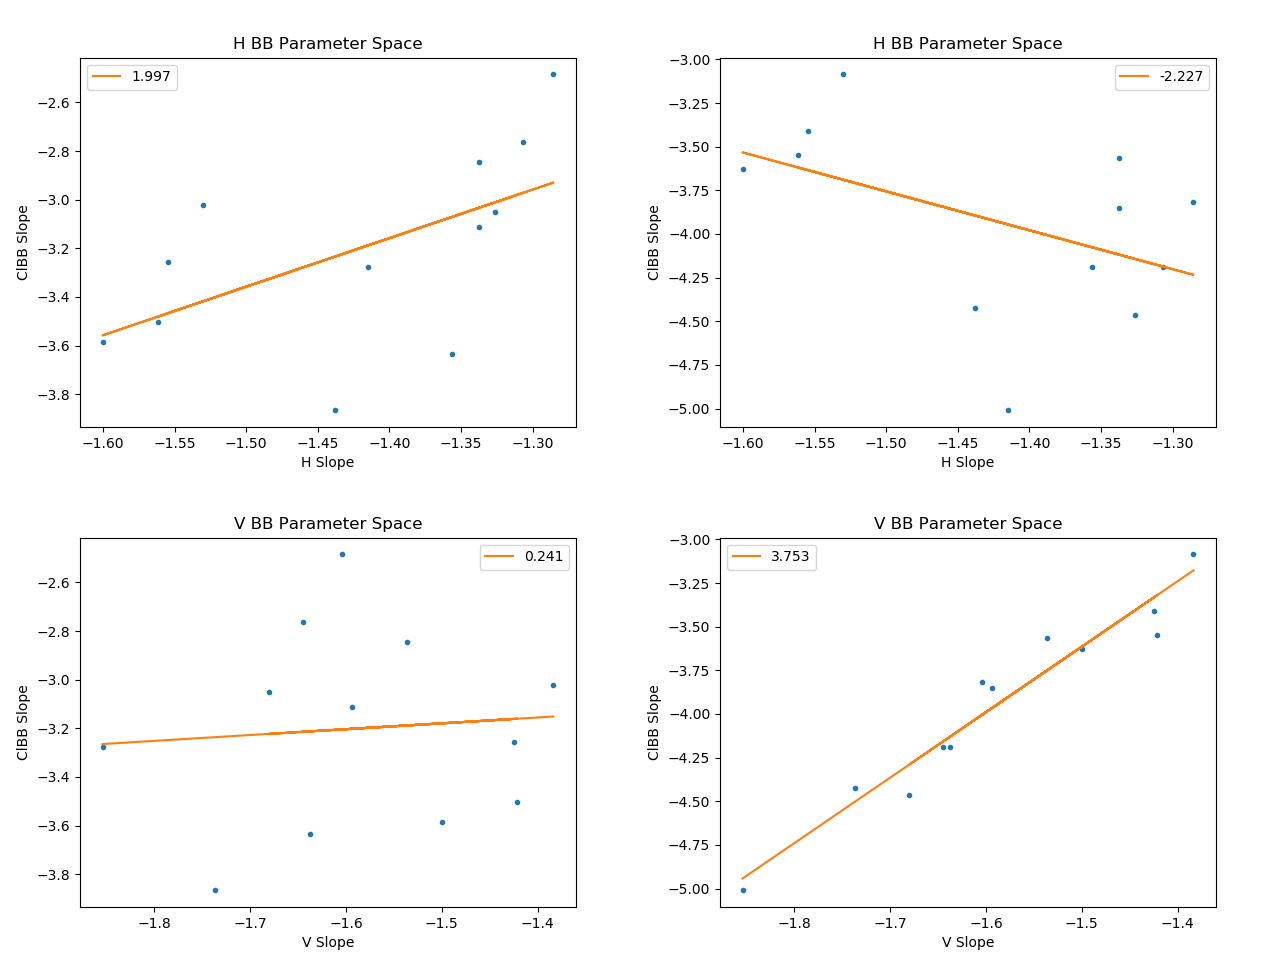
\includegraphics[width=\linewidth]{bb_V_H_x_y_paramspace.png}
\caption{Top Left: Slope of BB power spectra vs. slope of H-field spectra with
line of sight parallel to H-field. Top Right: Slope of BB power spectra vs.
slope of H-field spectra with los transverse to H-field. Bottom Left: Slope of
BB power spectra vs. slope of velocity spectra with los parallel to H-field.
Bottom Right: Slope of BB power spectra vs. slope of velocity spectra with los transverse to H-field}
\label{fig:bb_V_H}
\end{figure}

This line of sight effect on the power spectral slopes can be better understood
through figures ~\ref{fig:ee_V_H} and ~\ref{fig:bb_V_H}. These results clearly
demonstrate that for lines of sight along the magnetic field direction, the
shape of both the EE and BB spectra are closely correlated with the shape of
the magnetic field spectra and largely uncorrelated with the shape of the
velocity power spectra (left-most images in the figures). These figures also
demonstrate that the reverse is true when EE and BB are instead observed transverse to the magnetic field direction (right-most images in the figures).

\begin{figure}[h]
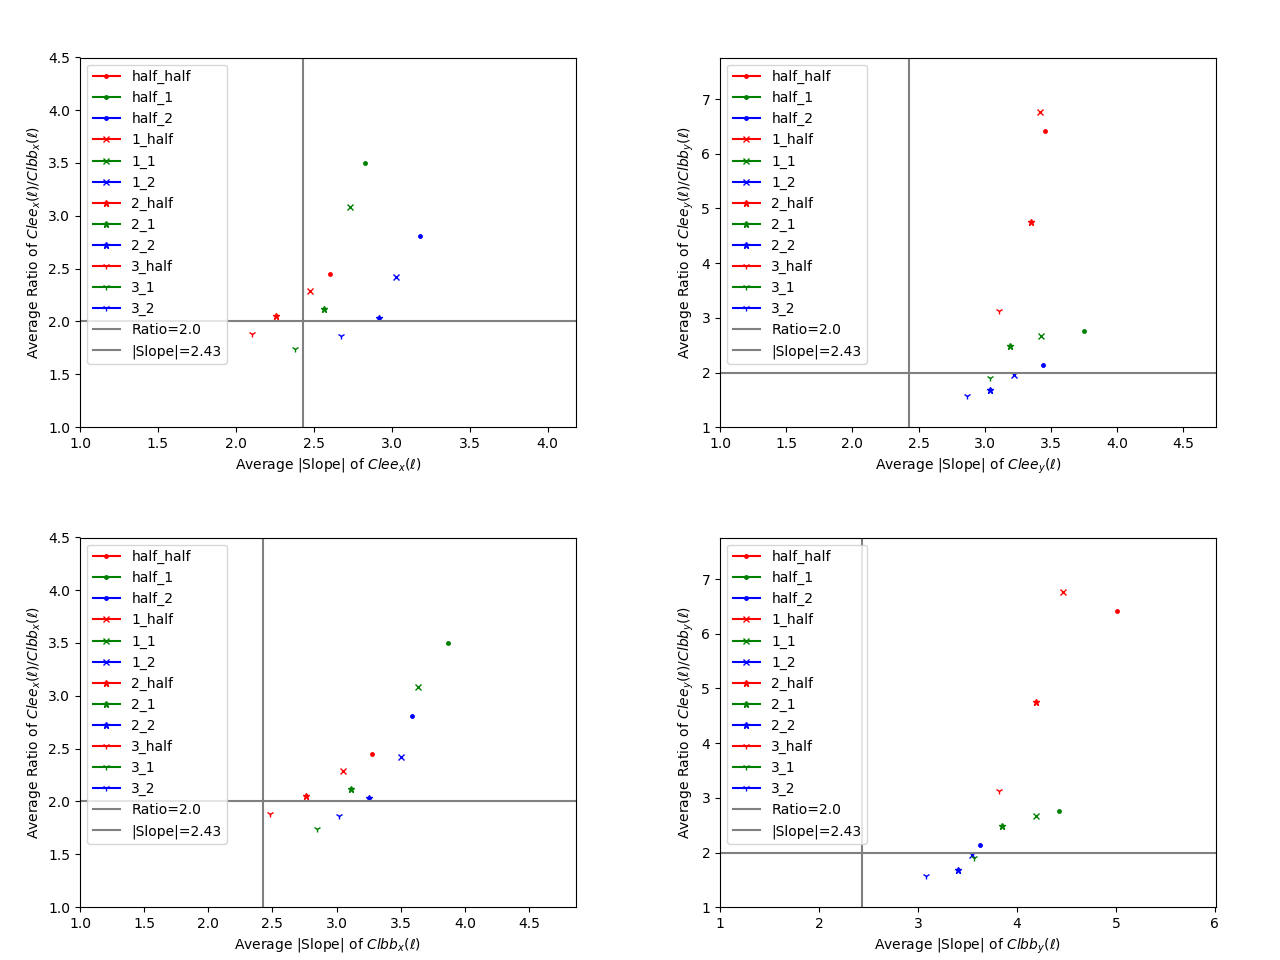
\includegraphics[width=\linewidth]{ee_x_y_bb_x_y_paramspace.png}
\caption{Top Left:Average E/B ratio $r$ vs Average EE slopes parallel to
magnetic field for all 12 simulations ran. Top Right: Average E/B ratio $r$ vs
Average EE slopes transverse to magnetic. Bottom Left: Average E/B ratio $r$ vs
Average BB slopes parallel to magnetic field. Bottom Right: Average E/B ratio
$r$ vs Average BB slopes transverse to magnetic field. All images have legends
labeled by $M_{s}\_ M_{a}$ associated with the simulation. Vertical and
horizontal grey lines in all images correspond to the $\alpha\approx-2.5$ and
$r\approx2$ respectively observed by \citep{Planck18XI}}
\label{fig:slopes_ratios_param}
\end{figure}

The main result of our survey and the overall effect that the above mentioned
correlations have on the observed slopes can be seen in figure
~\ref{fig:slopes_ratios_param} where we plot the observed EE and BB slopes
against their E/B ratios for all 12 of our various simulations. The horizontal
and vertical grey lines in the images represent the target E/B ratio
($r\approx2$) and target slope ($\alpha\approx-2.5$) respectively observed by
\citep{Planck18XI}.

With respect to $M_s$ and $M_a$ the slopes of EE and BB demonstrate two clear
properties. First for a given value of $M_a$, regardless of line of sight, both EE and BB have slopes that tend to become increasingly shallow as $M_s$ increases. This is
depicted in the figure by observing that for a given color ($M_a$), the order of
the symbols from left to right is the same in all cases and strictly decreasing
in sonic Mach number ($M_s$).

The second general observation on the spectral slopes of EE and BB that can be
seen in figure ~\ref{fig:slopes_ratios_param} encapsulates the line of sight
effects that we discussed earlier. For a given value of $M_s$, the spectral
slopes generally become shallower for \emph{increasing} $M_a$ when
measured \emph{transverse} to the background magnetic field. On the other hand,
for a given value of $M_s$ the spectral slopes generally become shallower for
\emph{decreasing} $M_a$ when measured \emph{parallel} to the background magnetic field.

With respect to the range of $M_s$ and $M_a$ used in our simulations, we find
that in general the highest sonic Mach number runs ($M_s=3$) tend to exhibit
slopes closest to our desired $\alpha\approx-2.5$ for any value of $M_a$. The
actual closest simulation to our desired result varies between lines of sight
and whether we look at EE or BB. It is therefore likely that the optimal $M_s$ value for the
desired slope occurs at a sonic Mach number beyond the range we tested here.
However our results do clearly suggest that a super-sonic, super-Alfvenic flow
is the most likely candidate for the EE and BB slopes observed. 




\section{E/B Power Spectra Ratios}

In this section we examine the ratio of power in the scalar EE spectra to the
tensor BB spectra across the inertial multipole range in our simulations.
We compare to the observed E/B ratio reported by \citep{Planck18XI} of
$r \approx 2$ and discuss the effects of various parameters on the value measured. 

\begin{figure}[h]
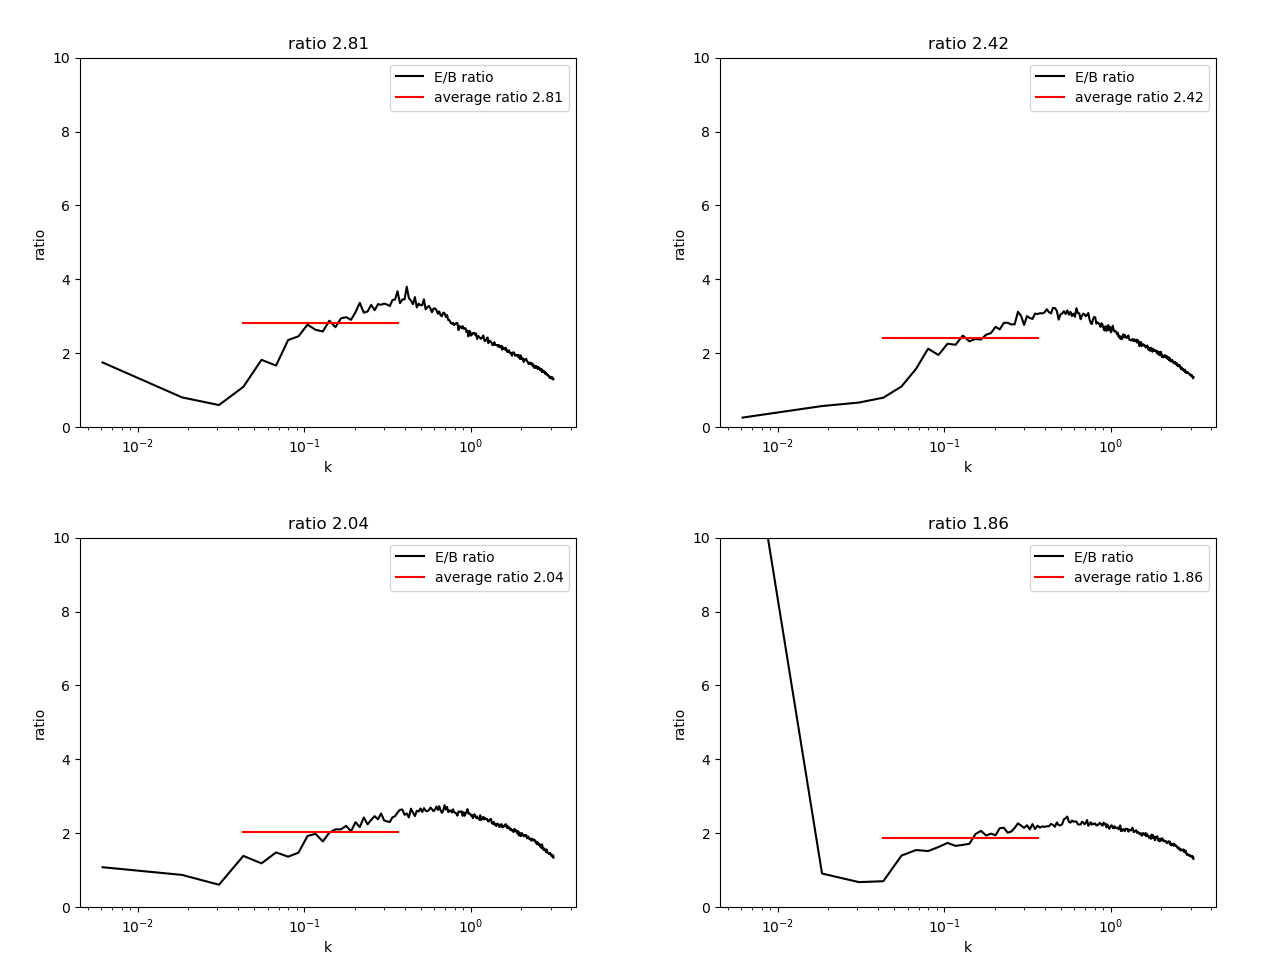
\includegraphics[width=\linewidth]{diff_ratios_x.png}
\caption{Average ratio of EE power to BB power EE/BB across the entire multipole
spectrum for four different simulations in our suite with varying $M_s$ and
$M_a$ parameters. Top Left: $M_s=0.5$ $M_a=2$. Top Right: $M_s=1$ $M_a=2$.
Bottom Left: $M_s=2$ $M_a=2$. Bottom Right: $M_s=3$ $M_a=2$. Each image is taken
with line of sight along the magnetic field and with a red horizontal line
depicting the average power ratio across the fitted inertial multipole range.}
\label{fig:ratio_ms}
\end{figure}

In figure ~\ref{fig:ratio_ms} we can explicitly see the effects of varying the
sonic Mach number $M_s$ on the observed E/B power ratio for a fixed, weak
background magnetic field. In these images we can see two features. The first is
that the ratio of E/B power \emph{decreases} as the ratio $M_{s} / M_{a}$
\emph{increases}. In other words as the sonic pressure increasingly dominates
the magnetic pressure, the ratio of power in EE to BB on average decreases. The
second feature, which is even more apparent in figure ~\ref{fig:ratio_ma} where
the gas pressure is held at a subsonic $M_s = 0.5$, is that the
power ratio as a function of multipole (size scale) becomes much more constant
(flat)  as the Alfven Mach number gets larger, that is to say as the magnetic field
pressure becomes less significant.

\begin{figure}[h]
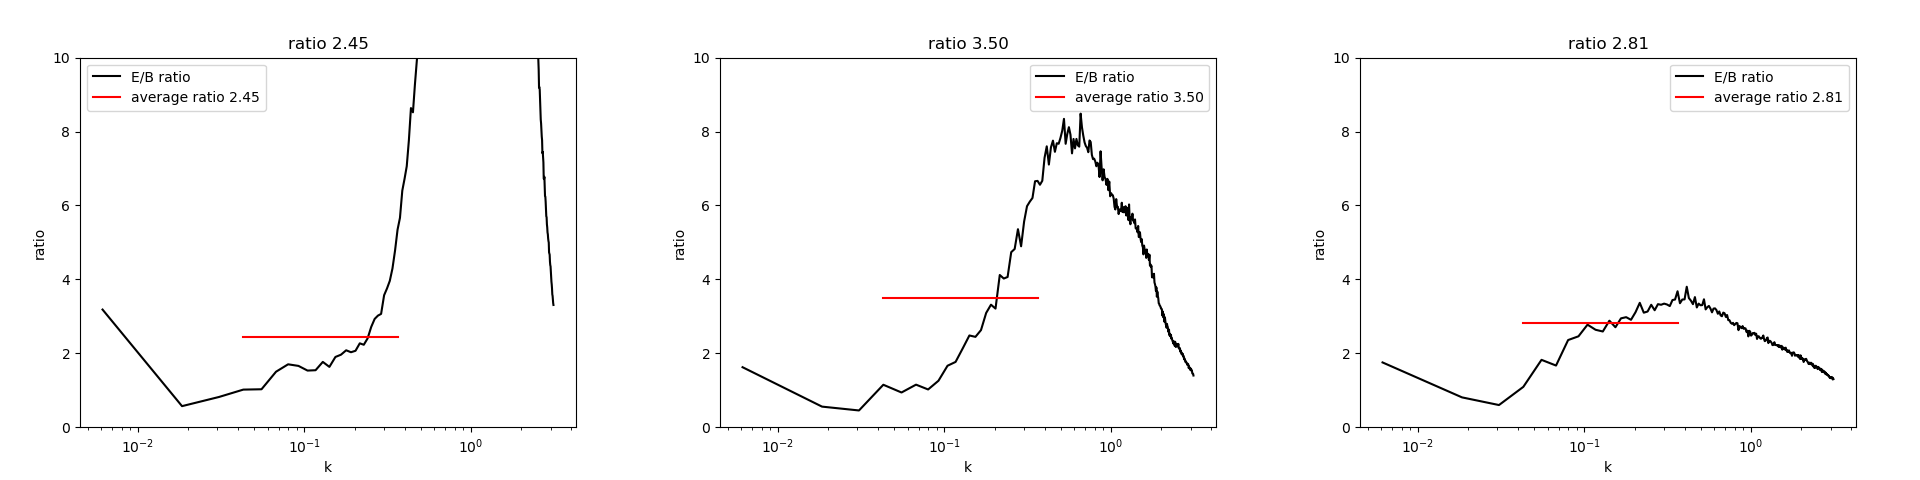
\includegraphics[width=\linewidth]{diff_ratios_x_Ma.png}
\caption{Average ratio of EE power to BB power EE/BB across the entire multipole
spectrum for three different simulations in our suite with varying $M_s$ and
$M_a$ parameters. Left: $M_s=half$ $M_a=half$.
Middle: $M_s=half$ $M_a=1$. Right: $M_s=half$ $M_a=2$. Each image is taken
with line of sight along the magnetic field and with a red horizontal line 
depicting the average power ratio across the fitted inertial multipole range.}
\label{fig:ratio_ma}
\end{figure}

Again the detailed results of our simulation suite including those discussed
above are most easily seen in figure ~\ref{fig:slopes_ratios_param}. Similarly
to the EE and BB slopes, we see that line of sight effects with respect to the
magnetic field orientation range from minimal, when the Alfven Mach number is
high (magnetic field is weak) to significant, when the Alfven Mach number is low
(strong magnetic field). Our results suggest that a super-sonic, super-Alfvenic
flow is the most likely candidate to explain the observed E/B ratios.


\section{T/E and T/B correlations}


\section{Conclusions}

Our simulations provide many insights into the possible nature of the polarized
dust foreground. We learned precisely how the slopes of the EE and BB power
spectra and EE/BB power ratios behave with respect to changing sonic and Alfven
mach numbers as well as observation orientation with respect to the background
magnetic field. We find that these values become increasingly non-isotropic with
respect to line of sight as the flow becomes sub-Alfvenic. 

These observations combined with a detailed parameter space analysis suggest that the
\citep{Planck18XI} results for EE and BB slopes $\alpha_{xx} \approx -2.5$ and
E/B power ratio $r \approx 2.0$ can most easily be explained by a super-sonic,
super-Alfvenic flow. If the dust is indeed sub-Alfvenic it will require a much
more super-sonic (or much more sub-Alfvenic) flow than those probed in this
project and the exact values of $M_s$ and $M_a$ able to probe the desired
parameter space would be much more strict.

In principle this narrowing of the allowed parameter space could be a good thing
since it would provide much more exact information into the allowed properties
of the polarized dust foreground, exactly what we are hoping to find. However
our results seem to suggest for now that so long as the flow is at least
moderately super-Alfvenic and super-sonic, a wide range of values for $M_s$ and
$M_a$ satisfy the observed parameters and isotropic nature.

Ultimately since a highly super-sonic flow in nature for these dust clouds is not unlikely,
it would be a valuable endeaver to run another suite of similar simulations with
greatly super-sonic, sub-Alfvenic conditions to see if these values are even
capable of achieving the desired parameter space our results suggest that they
might. 


%\input{acknowledgements}

%I'll probably cite \citet{Padoan02}
% Now I can cite  \citet{Kritsuk17}
%
%\begin{figure} \begin{center}
%    \includegraphics[width=0.49\textwidth]{Serkowski-LowerWavelength-Polarization-Paper08-B20-RS0050-x-_Stokes_HRO_Sigma.png}
%    \includegraphics[width=0.49\textwidth]{Serkowski-LowerWavelength-Polarization-Paper08-B20-RS0050-x-phi_cut.png}
%\caption[ ]{The figure on the Left is what? vs the right? }
%\label{} \end{center} \end{figure}

\bibliographystyle{apj}
\bibliography{apj-jour,ms.bib}  % looks in ms.bib for bibliography info

\end{document}  


